\documentclass[a4paper]{article}

\usepackage[utf8]{inputenc}
\usepackage[T1]{fontenc}
\usepackage{lmodern}
\usepackage[frenchb]{babel}

\usepackage{graphicx}
\usepackage{wrapfig}

\usepackage{amsmath}
\usepackage{amssymb}
\usepackage{chemfig}
\usepackage{cancel}

\usepackage{lettrine}
\usepackage{oldgerm}
\makeatletter
\@addtoreset{section}{part}
\makeatother

\begin{document}
\begin{center}
{\Huge \textbf{Projet TER RobotTaf}}
\\~
\\~
\\~
\\~
{\Large \textbf{Par:}}\\
\large{\textbf{Victor Coutellier - Julien Gauttier - Vladimir Karassouloff}}
\\~
\\~
\\~
\large{\textbf{Faculté des sciences d’Orléans -  M1 informatique}}
\\~
\\~
\\~
\end{center}

\tableofcontents
\newpage

\lettrine{L}'objectif de ce projet est de concevoir un mini langage servant à manipuler un robot afin d’enseigner les bases de la programmation aux jeunes enfants.
\\
Il s’agira de concevoir un langage de programmation contenant la plupart des notions de l’algorithmique et de le rendre accessible à des enfants. Une application Android devra être développer, les enfants devront alors créer un algorithme avec le langage préalablement conçu via cette application. Cette application servira d’interface entre l’enfant et le robot. Le programme produit par l’enfant devra ensuite être envoyé sur un robot qui lancera localement son exécution.

\section{Une introduction au domaine}

A l’origine, si l’apparition de la programmation à déclenché un élan d’apprentissage aux jeunes enfant, les premiers langages n’étais pas adaptées a ces derniers. En effet, la syntaxe était très exigeante et austère. De plus, la programmation était souvent introduite dans des contextes non familiers aux jeunes enfants, tel que la génération de nombres premiers, ou dessiner des formes géométriques.

\paragraph{}
Dans son livre \cite{Papert:1980:MCC:1095592}, Seymour Papert’s indique d’un language de programmation éducatif doit répondre à 3 critères
\begin{itemize}
\item « low-floor », c’est à dire simple d’accès
\item « high ceiling », c’est à dire fourni des opportunités de créer des projets complexe avec le temps
\item « wide-walls », c’est à dire suffisamment vaste pour engager different types de projets
\end{itemize}
Mais ces 3 contraintes n’étais pas satisfiables au vu des limitations techniques de l’époque.

\paragraph{}
Il est également remarqué d’une personne apprends mieux en travaillant sur des projets personnel, c’est pourquoi il est important d’insister sur
\begin{itemize}
\item La diversité des projets ( jeux, histoire, animations, simulations ), afin que chacun puisse se retrouver dans le langage utilisé
\item La personnalisation, il est donc important de pouvoir importer ses propres images, son, voix, ainsi que des outils pour créer ses propres ressources.
\item le choix de la 2D dans le développement d’une application d’apprentissage est donc plus approprié, car en effet, il est plus simple d’importer des assets 2D, tout comme il est plus simple de les personnaliser et de créer un environnement cohérents autour
\end{itemize}

\paragraph{}
Il fut également remarqué dans plusieurs études - notamment le département des sciences et de la technologie de l’éducation de l’université de Mons \cite{temperman:halshs-01092656}, et le Department of Psychologie of Nazarene College \cite{degelman1986concept} - que les enfants ayant été confrontés à des problèmes algorithmiques de façon ludique progresse de façon significative dans des problèmes mathématiques. Mais malgré cela, il fut aussi démontré que laisser l’enfant livré à lui-même dans un environnement de programmation ne suffit pas à developper ses capacités, le rôle de l’enseignant est primordial pour observer de réel effets positifs sur le développement de ces compétences.

\paragraph{}
« Si nous observons des gains d’apprentissage élevés dans le domaine des grandeurs, des nombres et de la structuration spatiale, l'impact du dispositif semble plus réduit pour les compétences relatives à la résolution de problèmes et pour le raisonnement logique. Un autre résultat intéressant qui ressort de notre analyse est l'effet du scénario en termes d’équité. Les résultats des apprenants sont en effet plus homogènes au terme de l’apprentissage. » \cite{temperman:halshs-01092656}  Indique l’étude de l’université de Mons.

\paragraph{}
Pour Seymour Papert, l’utilisation de l’ordinateur de manière éducative afin de créer des object, dessins, ou programme via un environnement adapté devient un catalyseur pour un changement positif dans le parcours scolaire de l’enfant \cite{clements1999young}.

\section{Une analyse de l’existant}
\subsection{Le système LOGO}

\paragraph{}
Cet article \cite{mendelsohn1985enfant} parle de l’évolution de l’enseignement assisté par ordinateur et de ses différentes approches tel que des didacticiels, des simulations, apprentissage des différents langages. En effet, il s’agit d’une approche ludique pour les enfant avec résolution des problème et exploration de la géométrie grâce a une mise a disposition de différents élément, ici avec Logo, on dirige une tortue que l’on déplace à l’aide de divers fonctions munies d’arguments pour effectuer des opérations (exemple : av 150 td 120 av 150 td 120 av 150 dessinera un triangle)

\paragraph{}
L’apprentissage de la programmation passe par l’apprentissage de la logique pour maîtriser les algorithmes. On remarque également que la programmation peut aussi apprendre dans d’autre domaines tel que la musique, calcul, etc…

\paragraph{}
Parle des avantages de la pratique de la programmation
\begin{itemize}
\item Permet d’aborder des concepts difficile a aborder tel que la récursivité, les variables
\item Capacité de prévoir le résultat lors d’une suite de diverse transformation d’un objet
\item Découverte du concept d’automates
\item Augmentation de la capacité a résoudre des problèmes
\end{itemize}

\paragraph{}
Logo permet d’acquérir de l’expérience réelle sur objets de connaissance à travers des concepts tel que
\begin{itemize}
\item Le concept d’état (le fait que la tortue repérable sur l’écran par sa position et sa direction)
\item Les commandes qui permettent de changer l’état de la tortue
\item La transposition de la tortue dans le monde réel via des système robotique, permettant à l’enfant de ressentir directement les effets de son travail
\end{itemize}

\paragraph{}
Les enfants apprécient la possibilité de personnaliser les programmes en donnant les nom qu’ils veulent aux variable / fonctions. C’est un véritable “laboratoire d’apprentissage et de recherche” mise à disposition de l’enfant.

\subsection{Le langage Squeak Etoys}

\paragraph{}
Squeak Etoys \cite{kay2005squeak} est un logiciel inspirée par LOGO, il s’agit d’un environnement de développement qui inclue des graphismes 2D et 3D, des images, textes, particules et permet même des pages web ou des clips vidéo. Cet environnement permet également de partager ses créations en temps réel avec d’autres utilisateurs à travers le monde. C’est un système gratuit, open source et multiplateforme.

\paragraph{}
Tout dans Squeak est considéré comme un objet, et l’on peut ajouter des contraintes et donner des instructions à tout ces objets. En effet, l’interface est des plus minimalistes pour ne pas submerger l’utilisateur par des dizaines de boutons et d’options, afin de laisser l’enfant découvrir le logiciel à son rythme sans être intrusif sur ce qui est considéré comme fait ou à faire.

\paragraph{}
Squeak fusionne la notion de « zone d’édition » et de « zone de rendu », en effet, tout les objets sont modifiables à la volée lors de l’exécution du projet. Cela permet de clarifier l’interface dans le sens ou il n’existe qu’un seul contexte, celui de la page principale. Des bulles d’aides apparaissent tout de même avec un certains délais afin de guider l’utilisateur sur les informations utiles en fonction de sa sélection \cite{yatim2007educating}.

\paragraph{}
De part ces mécaniques, Squeak permet à l’utilisateur final d’accéder à la simplicité sous-jacente de different concept important tel la gestion du son ou des images.

\subsection{Le langage Scrath Junior}

\paragraph{}
Scratch à été conçu afin  de permettre de programmer à des personnes qui n’ont jamais été amené à une carrière de développeurs. Il a été désigné pour tout le monde, de tout âges, afin de créer des jeux, simulations, animations ou histoire interactives \cite{Maloney:2010:SPL:1868358.1868363}.

\paragraph{}
Le but de cette plateforme n’est pas de former des programmeurs professionnels mais bel et bien de permettre à des personnes de tout horizons d’exprimer leurs idées \cite{resnick2009scratch}. En effet, de nombreuses personnes jouent à des jeux vidéos, regardes des animations ou utilisent des logiciels, mais peut on l’occasion d’en créer, et c’est cette opportunité que donne Scratch, ces compétences ainsi acquises peuvent être transposées dans des domaines qui n’ont rien à voir avec l’apprentissage ou l’utilisation de la programmation.

\paragraph{}
En effet, certains langages permettait déjà ces possibilités, tel que Squeak Etoys ou Alice, mais scratch était destiné à pousser encore plus loin l’accessibilité et les possibilités \cite{resnick2009scratch}.

\paragraph{}
Scratch fut conçu via les 3 principes suivant :
\begin{itemize}
\item Le rendre le plus flexible
\item Le rendre plus riche de sens pour les jeunes enfants
\item Le rendre plus social qu’un environnement de programmation traditionnel
\end{itemize}

\paragraph{}
Scratch est conçu comme de manière graphique \cite{resnick2009scratch}. En effet, aucune syntaxe n’est présente, les structures de données et de contrôles traditionnelles sont remplacées par des forme géométriques tel les pièces d’un puzzle. Par exemple, une boucle sera présenté en forme de C, de manière à pouvoir placer des blocs à l’intérieur afin de visuellement expliciter le concept de suite d’instruction se répétant.

\paragraph{}
Cette visualisation graphique permet donc à un enfant d’expérimenter toute sortes de combinaisons, tout cela couplé à une exécution des plus simples, en effet, le simple clic sur un élément déclenche son code dans l’application, il est même possible de modifier une séquence d’instruction à la volée pendant son exécution.

\paragraph{}
L’interface de scratch est prévu comme un bureau physique \cite{resnick2009scratch}, des instructions peuvent ainsi être disséminée ici et la sans lien les unes envers les autres afin d’être réutilisées par la suite en cas de besoin. Ce mode de fonctionnement incite donc à la découverte et à l’expérimentation plus qu’un langage de programmation traditionnel, qui implique rigueur et une conception préalable.

\paragraph{}
Une extension physique de Scratch existe, la Scratch PicoBoard, qui permet aux projet Scratch d’interagir avec le monde extérieur via une batterie de capteur, tel un capteur de luminosité, un bouton, un potentiomètre et même un micro, afin de rendre les projet plus interactif et plus palpable par l’utilisateur \cite{resnick2009scratch}.

\subsection{Le système LEGO Mindstorm}

\paragraph{}
LEGO Mindstorm est une gamme de la marque LEGO basée sur le concept de « brique programmable », c’est une brique qui permet de charger et d’exécuter des programmes utilisant toute une batterie de capteurs et d’actuateurs. Il devient donc très simple de créer un robot capable de se déplacer, d’attraper ou de reconnaitre des objets. \cite{martin1993lego}

\paragraph{}
Cette approche de la programmation par la robotique est des plus enrichissante, car l’aspect programmation pur est distillé par tout l’aspect ludique de la construction de son propre robot, tout en recevant des feedback physique à partir de son travail \cite{weinberg2003robotics}. Seymour Papert, déjà un des pionnier du langage LOGO, nomme cette pratique d’apprentissage de la programmation par des plateformes robotique le « constructionisme » \cite{Papert:1980:MCC:1095592}

\paragraph{}
Le second facteur de l’adoption des robots dans l’apprentissage de la programmation est la chute du prix du matériel nécessaire sur la dernière décennie. Il est en effet très bon marché même pour les écoles les plus modestes d’accéder aux composant nécessaires. Car même si ces composant ne fournissent pas la précision nécessaire à un usage industriel, ils sont largement suffisant pour un usage éducatif.

\subsection{Les systèmes annexes}

\paragraph{}
Ardublock est un programme de développement pour l'arduino a base de blocks. Cet outils à été testé sur des enfants et montre que l'apprentissage de la programmation en utilisant arduino est possible et qu'une évolutions dans certains domaines tel que la résolution de problèmes ont été observées chez les enfants.  \cite{sohn2014design}

\paragraph{}
https://www.aldebaran.com/fr/cool-robots/nao/en-savoir-plus-sur-nao : robots existants possèdant plusieurs capteurs afin d’interagir avec son utilisateur, on notera surtout la présence de capteurs pour se repérer, la possibilité de se mouvoir ainsi que la présence d’une carte wifi/ethernet.

\section{Une liste et analyse des besoins non-fonctionnels}
\subsection{Prototype test}
Télécommande : sera utile aux tests. En effet, le simple fait de contrôler le robot via une télécommande permet de vérifier plusieurs points. D’une part, cela permet de tester le fonctionnement et les capteurs du robot, et d’autre part, cela permet de se familiariser avec la “chaine d’action” du projet. Enchaînant l’application android, la production du code en mini-language, la communication avec le robot, la compilation sur ce dernier et son exécution. Cela sera donc la première étape du projet.

\subsection{Architectures}
Nous avons imaginé ici différentes architectures possibles, elles diffèrent de par leur facon de transcrire notre pseudo code en Arduino, l’acheminement de la sortie pseudo code de l’application Android jusqu'à son exécution sur le robot peut en effet se voir de différentes manières.
\subsubsection{Erlang}

\begin{center}
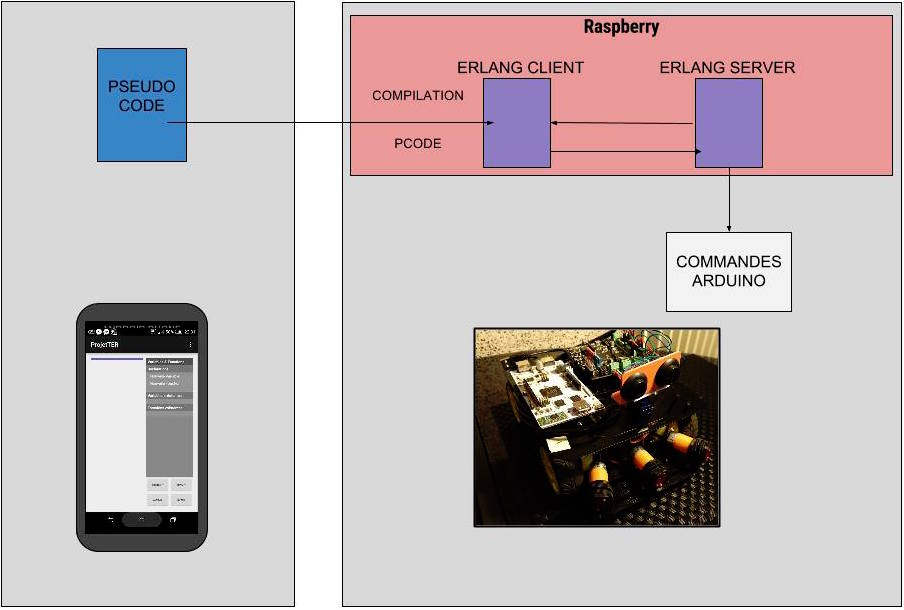
\includegraphics[scale=0.5]{img/archi-erlang.jpg}
\end{center}

Cette méthode profite de la facilité de communication entre plusieurs processus dont dispose Erlang, elle s’avère en premier lieu simple d’implémentations, on pourrait également se demander si une telle architecture ne serait pas simplifiable, et si nos commandes Arduino ne pourraient elles pas découler directement de la compilation.\\
Le PCode nous sers de langage machine, en effet, ce langage proche de l'assembleur nous permettrait de l'interpreter en commande erlang directement éxécutable par le robot.

\vfill\eject
\subsubsection{Pcode}

\begin{center}
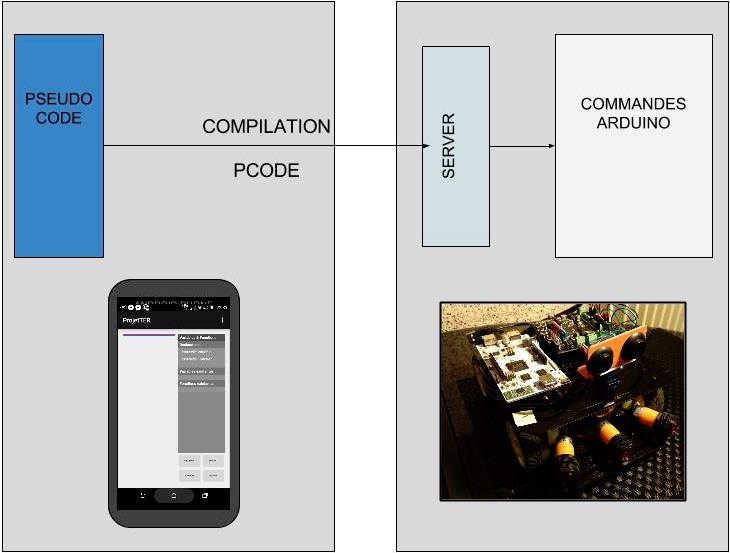
\includegraphics[scale=0.5]{img/archi-pcode.jpg}
\end{center}

Avec cette méthode on allège le cheminement du code, mais on perd le coté pratique de Erlang, c’est une façon plus directe, on passe de notre pseudo code à des commandes Arduino avec plus de transparence. On se sers la encore du PCode comme langage machine intermédiaire, c'est ce PCode qui est interpreté directement par l'Arduino.

\vfill\eject
\subsubsection{Lua}

\begin{center}
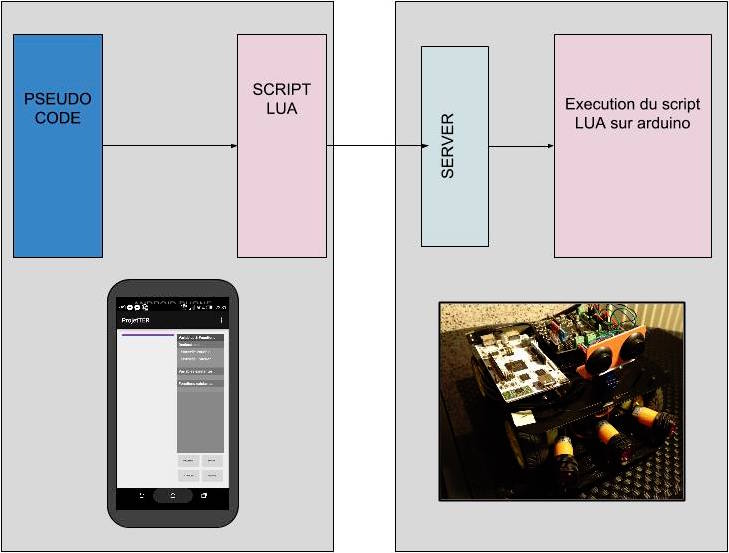
\includegraphics[scale=0.5]{img/archi-lua.jpg}
\end{center}

Cette architecture est basée uniquement sur la capacitée de la carte arduino à recevoir une implementation de LUA Script, si la carte controleur peut éxécuter une version basique de LUA, il est donc possible de directement envoyer un script LUA sur l'arduino, et ce dernier l'éxécutera sans problème sans autre forme de compilation.\\
La seul tâche à effectuer sera de transformer le pseudo code issu de l'interface de l'application android en LUA Script.

\section{Une liste et analyse des besoins fonctionnels}

\subsection{Application}

L’application Android servira à construire un algorithme à travers une interface utilisateur imaginée pour les enfants.

\paragraph{}
L'interface utilisateur de l'application est pensée pour les enfants, il necessite donc de ne pas afficher directement du code face à l'utilisateur, mais plutôt des blocs s'imbriquant les uns les autres pour former un programme. Il est également necessaire d'insister sur les formes et les couleurs afin de rendre l'application ludique pour l'utilisateur. En effet, toutes les combinaisons de blocs possibles qu'offre l'application doivent être éxécutables, afin que l'enfant puisse comprendre directement les conséquences de ses actions, et non se confronter à des erreurs.

\paragraph{}
Les principales inspirations pour l'application fûrent notamment l'application LEGO EV3 et Scratch JR pour tablette, ou les programmes sont composées de blocs tel des pieces d'un puzzle, ou chaque bloc est utilisable independamment et représente une action. Ces deux applications montrent une fenêtre principale dite de "bureau", c'est à dire la fenètre ou l'utilisateur peut faconner librement son programme, en imbriquant les briques les unes avec les autres pour former un algorithme complet.\\
Sous cette fenètre de bureau se trouve un système d'onglet, et chaque onglet correspond à une catégorie de blocs representant une action. Par exemple l'onglet des capteurs proposera des blocs pour lire la valeur de tel ou tel capteurs, l'onglet des actuateurs contiendra des blocs pour actionner les moteurs, jouer un son ou emettre de la lumière.\\

\paragraph{}
Dans l'application LEGO EV3, un onglet flux permet de catégoriser les blocs controlant le déroulement de l'application, on y retrouve donc un bloc "debut" symbolisant le début du programme, ou un bloc "repeter", en forme de C afin de montrer que ce bloc n'est qu'un conteneur pour placer d'autres blocs d'action à l'interieur. Chaque bloc est ainsi personnalisable pour en limiter le nombre de base. Par exemple le bloc "jouer un son", une fois placé dans le programme, va permettre de choisir quel type de son jouer, et à quelle intensitée pendant combien de temps.

\paragraph{}
Dans l'application Scratch JR, étant plus adaptée aux enfants, on remarque la possibilitée d'importer et de modifier ses propres images et son depuis la tablette, afin d'offrir des capacités de personnalisation poussée du programme, pour que l'enfant s'identifie plus au projet. Il est également necessaire que l'espace de travail sois perçu comme un bureau physique, ou l'on peut laisser des blocs de côté, afin d'être réutilisé plus tard, ou seul les blocs colés après le bloc "debut" sont pris en compte dans l'éxécution finale

\subsection{Robot}

\begin{center}
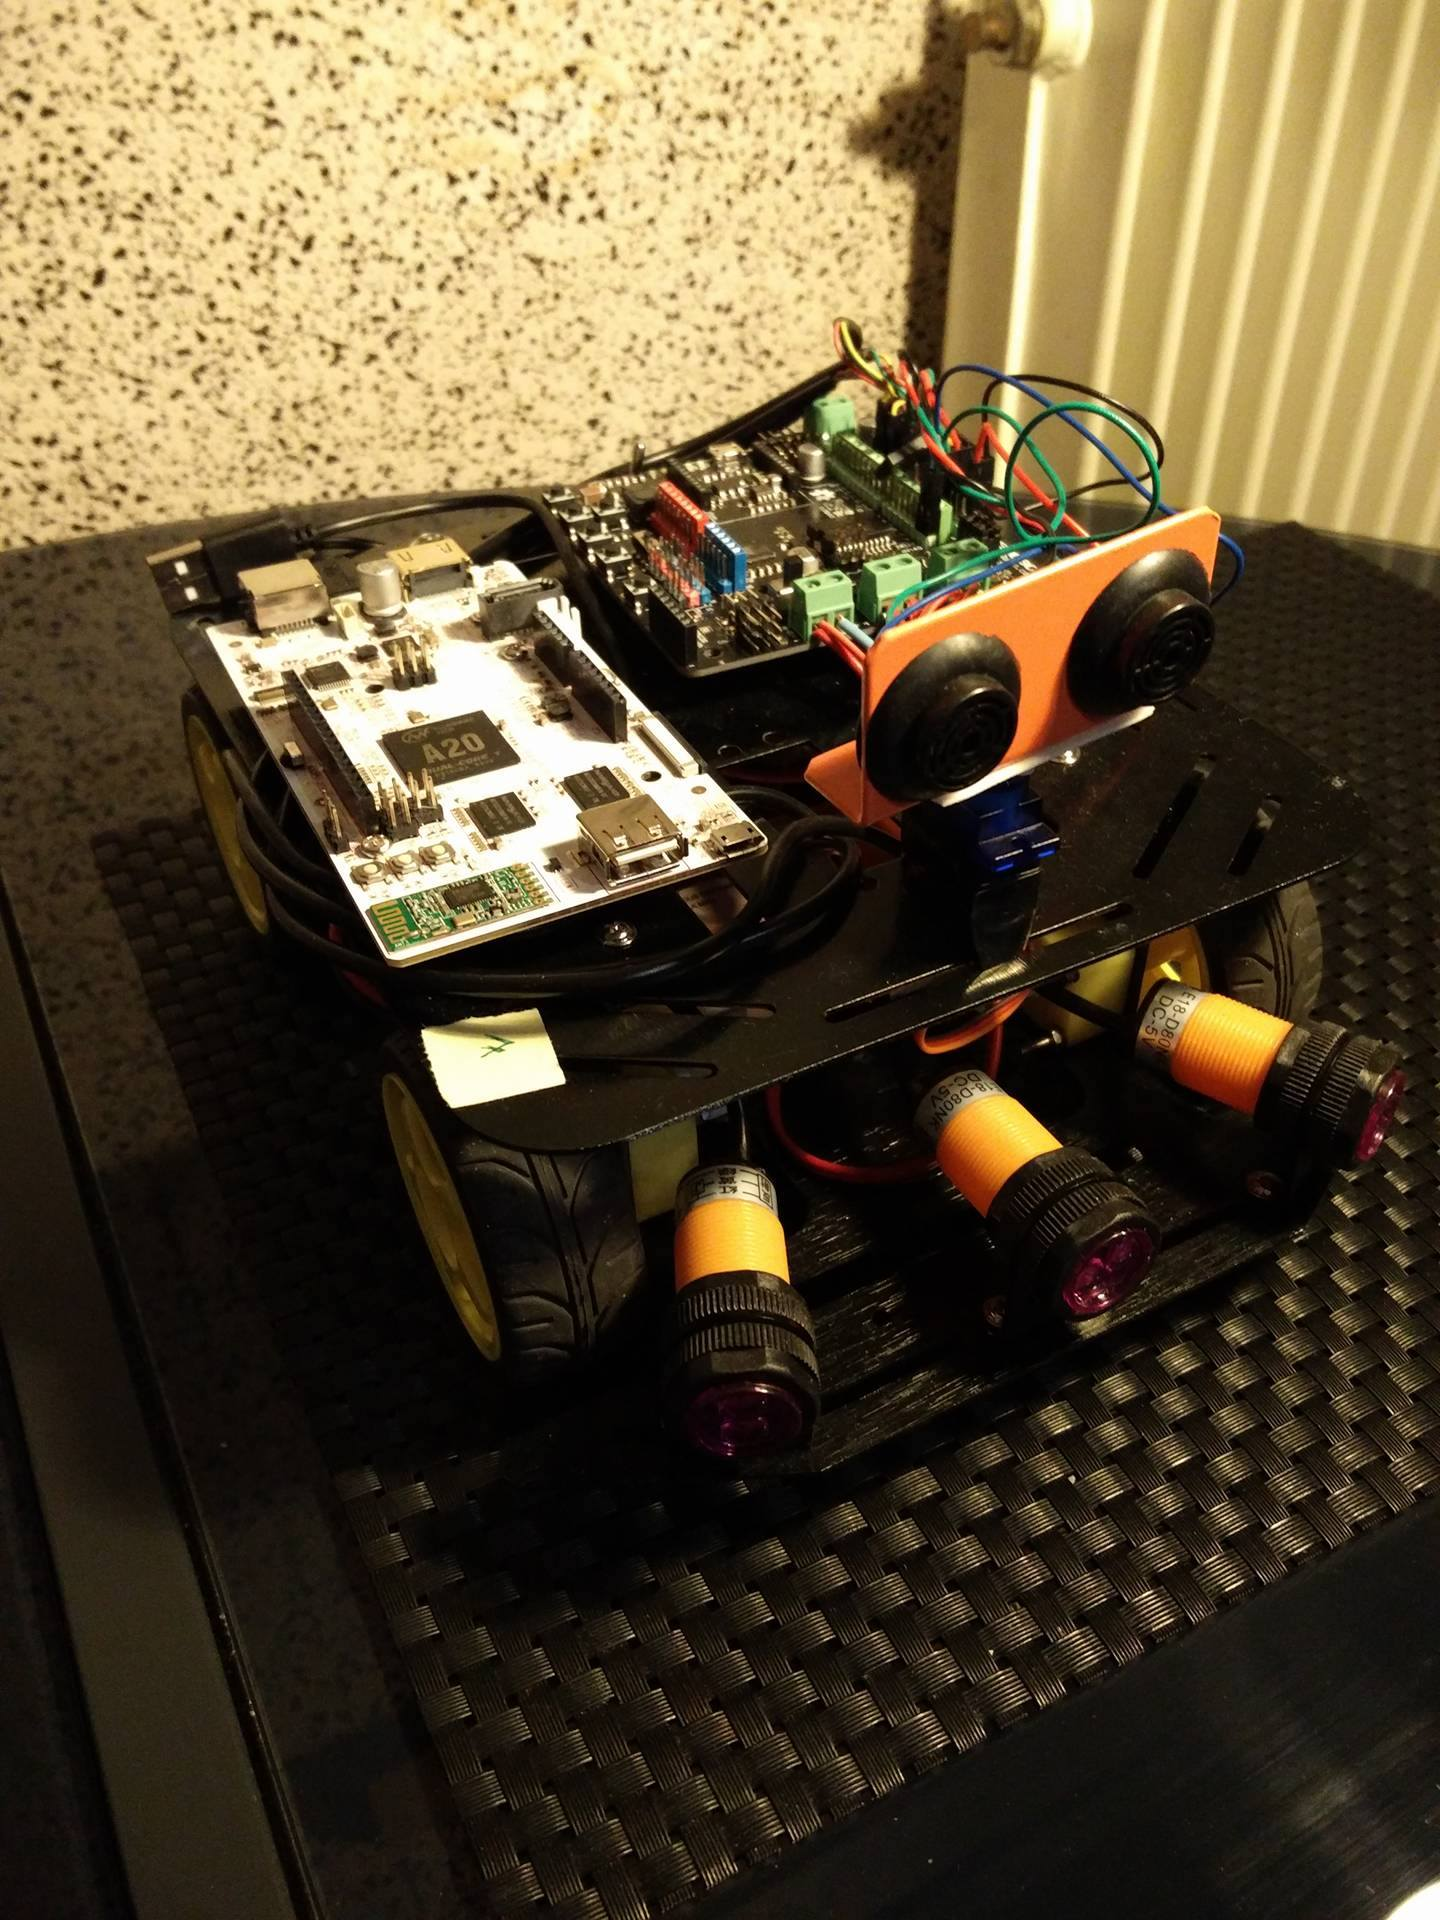
\includegraphics[scale=0.15]{img/robot.jpg}
\end{center}

\paragraph{}
Le robot est, dans le cadre du projet, composé :
\begin{itemize}
\item D'un chassis à 4 roues motrices, sur lequel viens se fixer les differents capteurs, moteurs et carte élétroniques
\item De 4 roues motrices actionnés par une batterie externe pour délivrer plus de puissance
\item D'un capteur à ultrasons, posté sur un servo-moteur
\item De 3 capteurs de proximités infrarouges
\item D'une carte controleur de type Romeo, basée sur un Arduino Leonardo
\item D'un mini pc tel un raspberry pi, avec wifi et bluetooth, fonctionnant sous ubuntu qui est relié en USB à la carte contrôleur
\item De deux batterie, une pour la carte contrôleur et le mini pc, l'autre spécifique pour les moteurs
\end{itemize}

\paragraph{}
Le but du robot est de communiquer en direct avec l'application Android via Wifi, afin de recevoir le code produit par l'utilisateur sur l'application, et selon l'architecture choisis de directement l'éxécuter sur l'arduino, ou de préalablement recompiler ce code pour l'éxécuter ensuite.\\
Il sera par la suite possible d'améliorer ce robot afin d'ajout differents capteurs, ou même de se passer du mini pc si les instructions passée à l'arduino sont déjà pré-compilées par le téléphone afin de les envoyer directement à la carte contrôleur via un shield Arduino Wifi, cela baisserait drastiquement la taille et le coup de production du dit robot.

\subsection{Mini-Langage}

Le développement d’un mini-langage est crucial dans ce projet, en effet, l’application ne sers que d’interface pour facilement écrire ce langage, qui sera traduit de manière formelle via l’application. Ce langage formel, défini via une grammaire, subira plusieurs phases d’analyse soit : lexicale, syntaxique et sémantique, afin de traduire ce mini-langage dans un langage machine exécutable sur le robot afin d’effectuer les requêtes de l’utilisateur.

\paragraph{}
Ce mini-langage sera une interpretation du "bureau" de l'application, c'est à dire de la suite de blocs prise en compte dans le programme final. Le langage cible sera donc une serie de commande très simple, envoyée sur le port serie de l'Arduino ou directement via wifi si une architecture sans mini pc est choisie, afin que ces commandes sois directement comprise et éxécutées via le code de la carte controlleur arduino.

\section{Une description de prototypes et des résultats de tests préparatoires}
\subsection{Prototype android}
\begin{center}
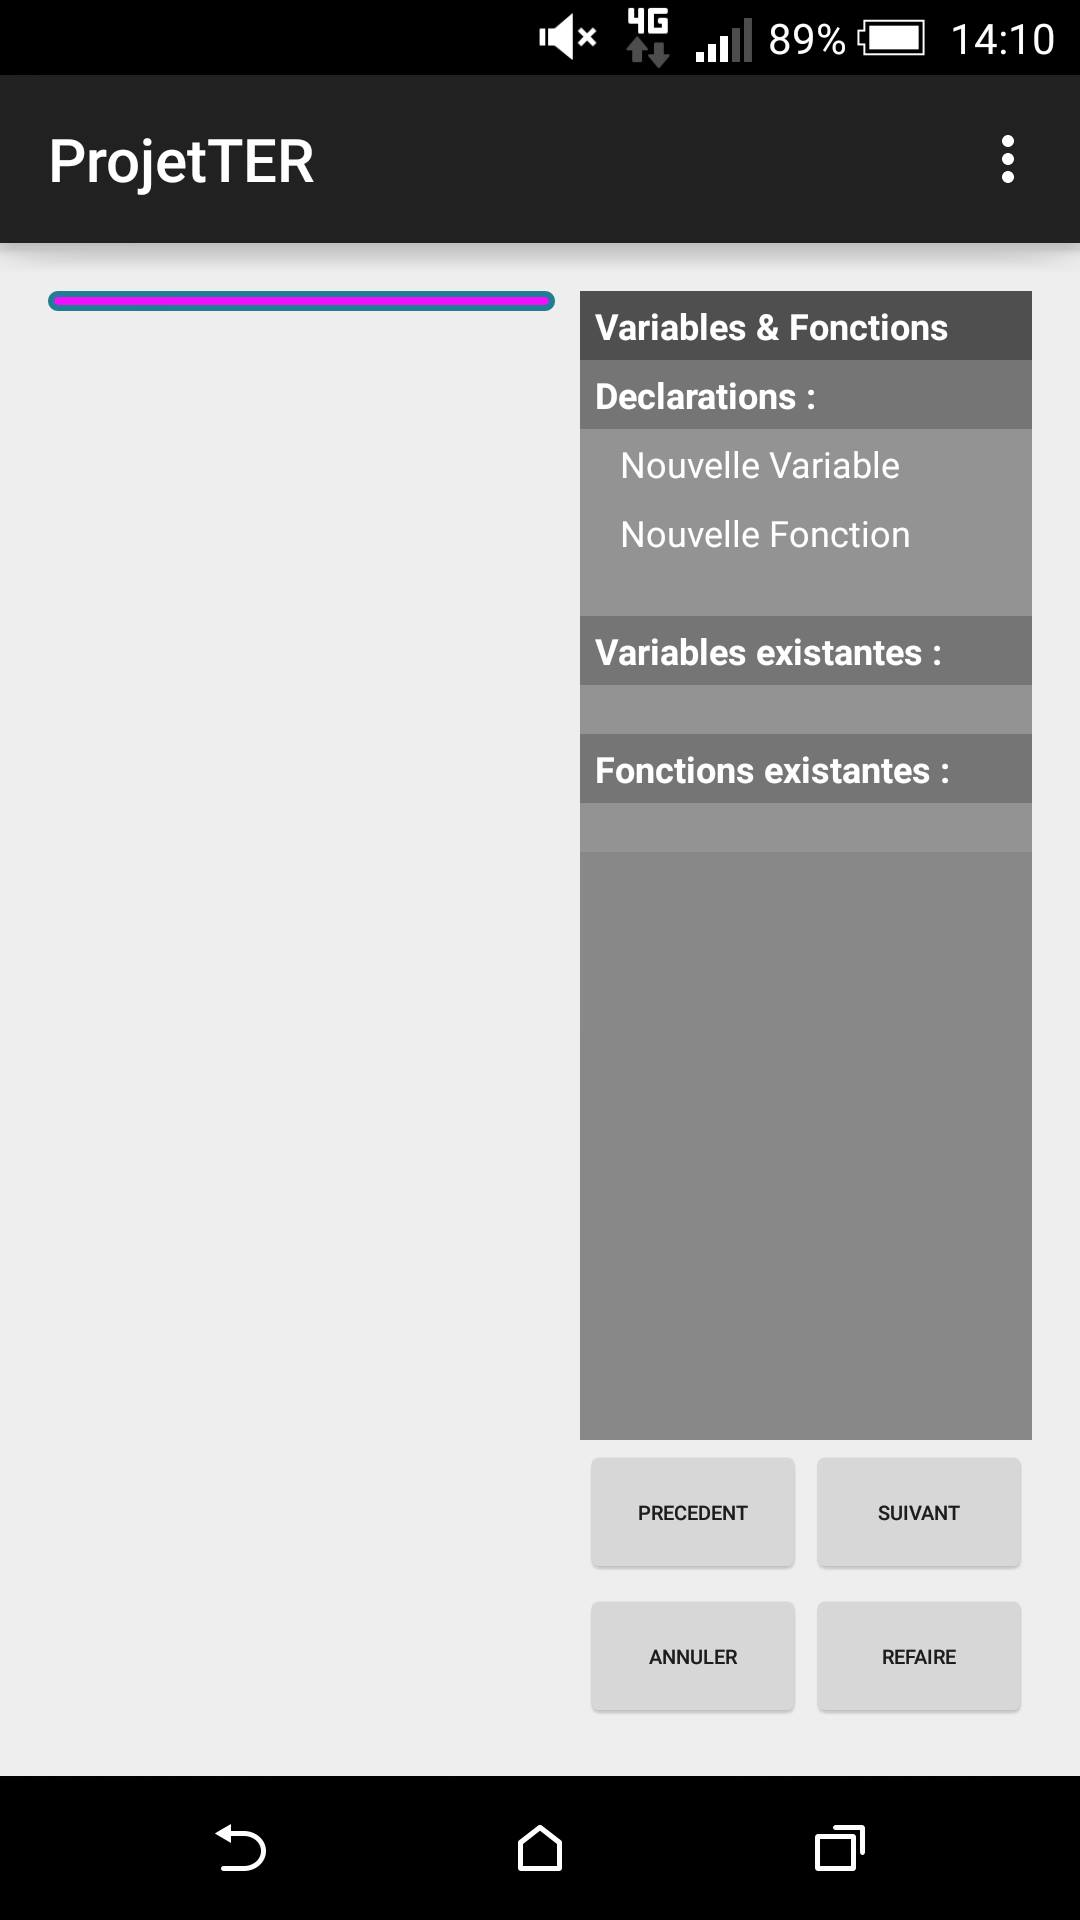
\includegraphics[scale=0.1]{img/menu_variableFonctions.jpg}
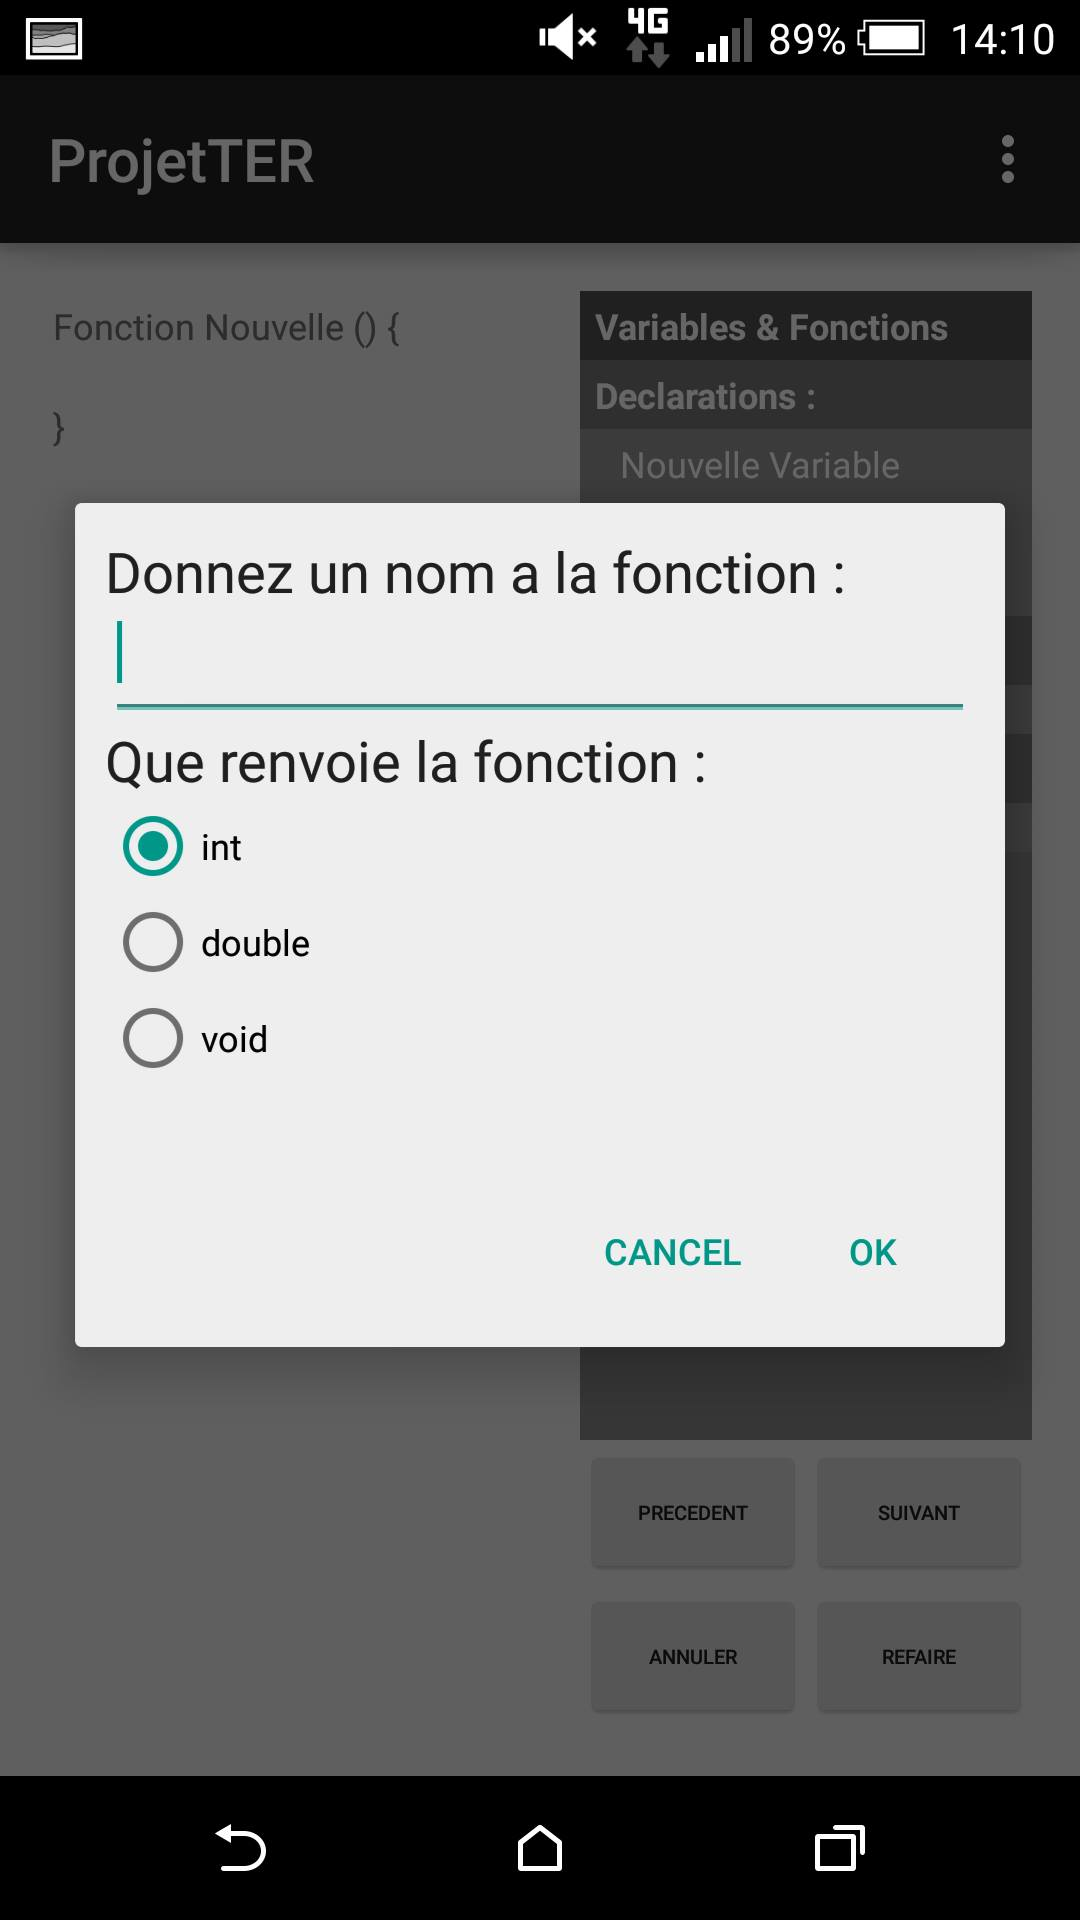
\includegraphics[scale=0.1]{img/popup_fonction.jpg}
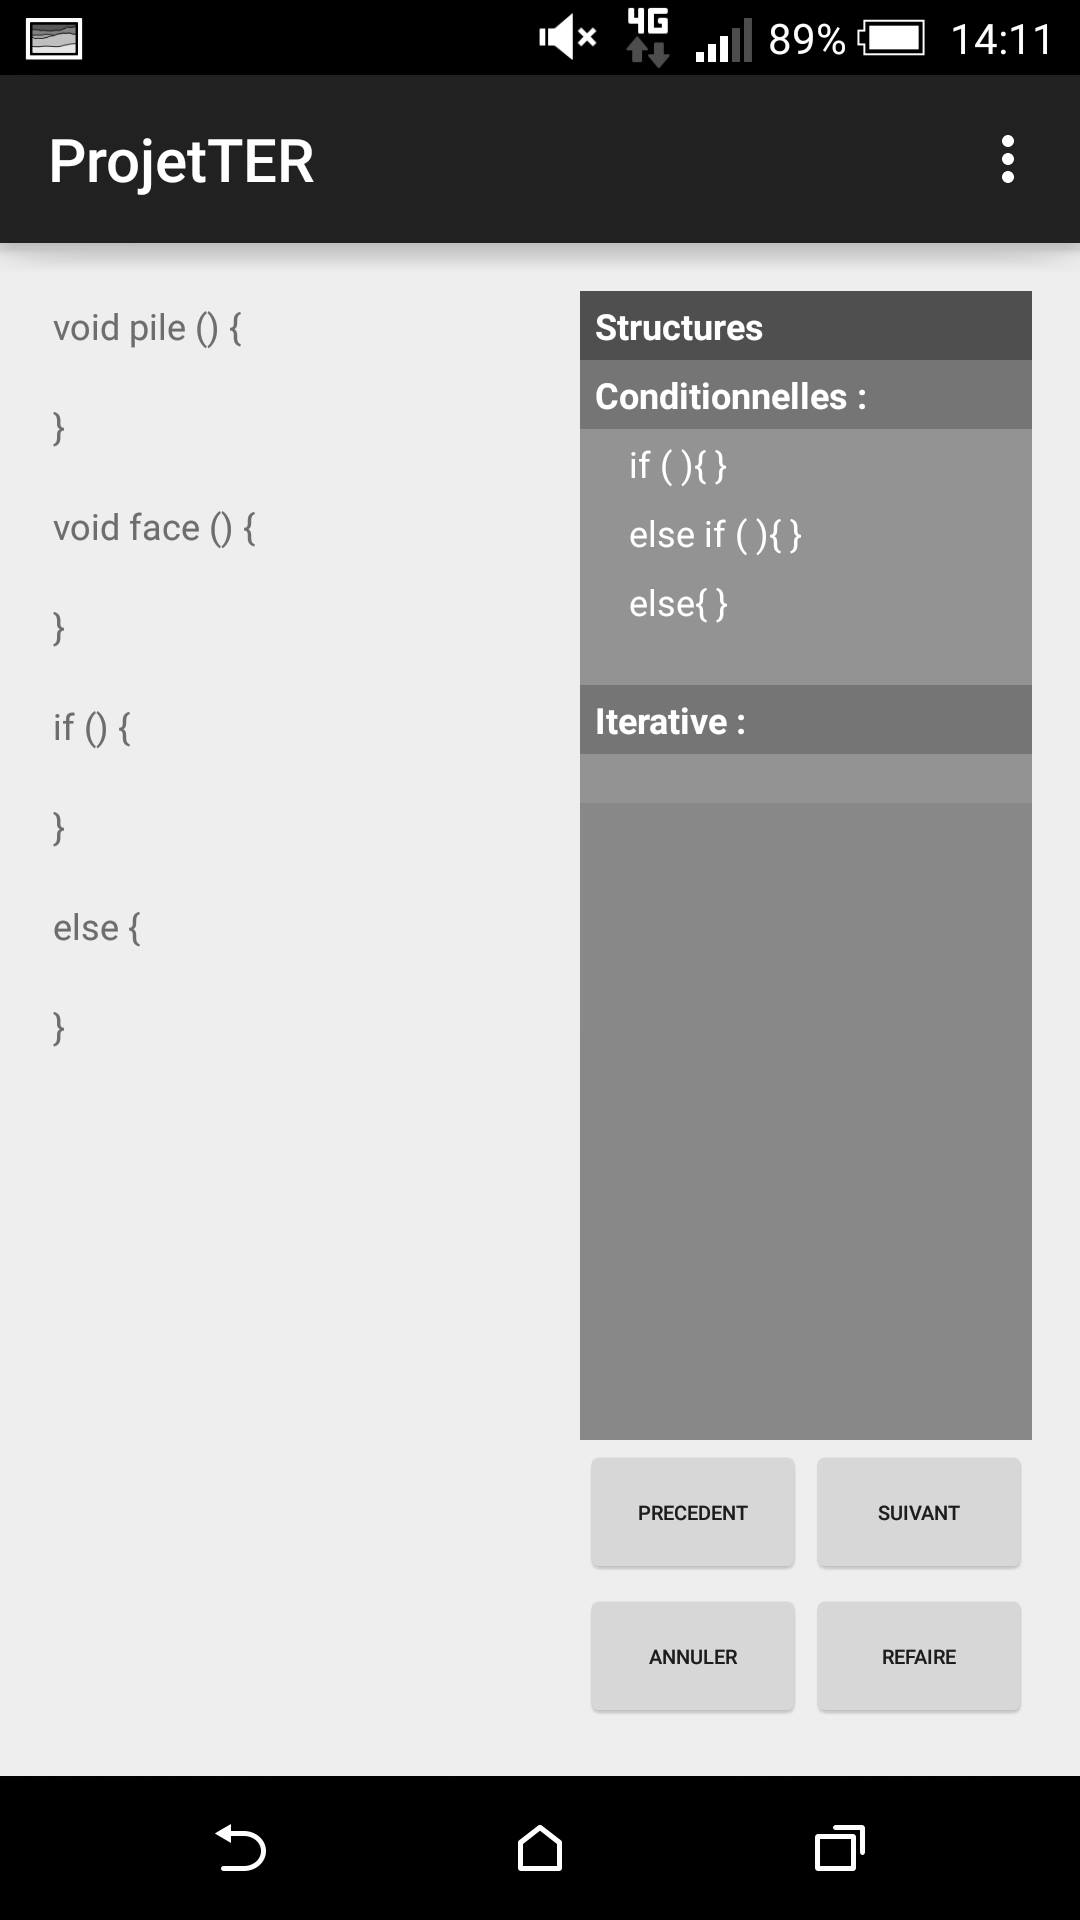
\includegraphics[scale=0.1]{img/create1.jpg}
\end{center}
Une Viewanimator à droite, contenant liste de scrollview contenant différents élément de programmations tel que les structures (conditionnelles et boucles), les variables ou encore les opérateur de calculs et logique. Les différents éléments peuvent être drag and drop vers d’autres vues. \\
\\
\begin{center}
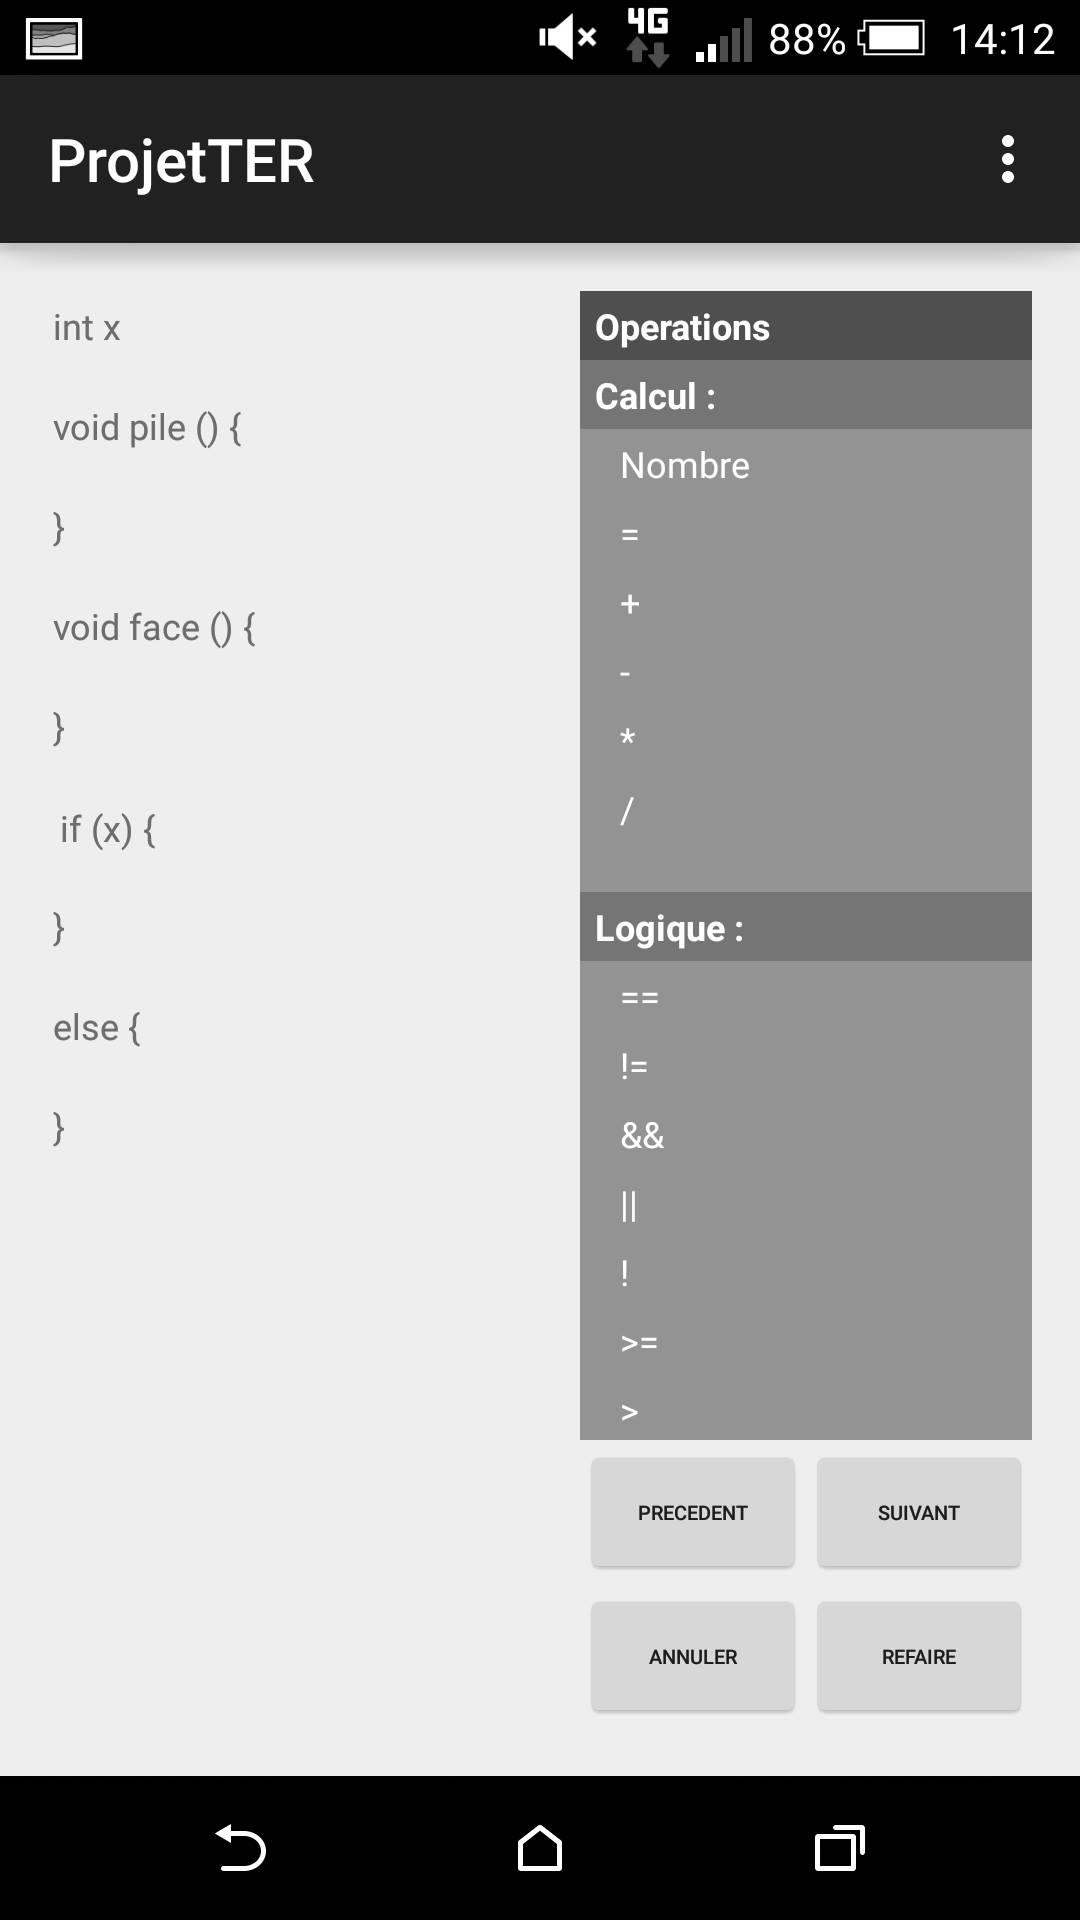
\includegraphics[scale=0.1]{img/create2.jpg}
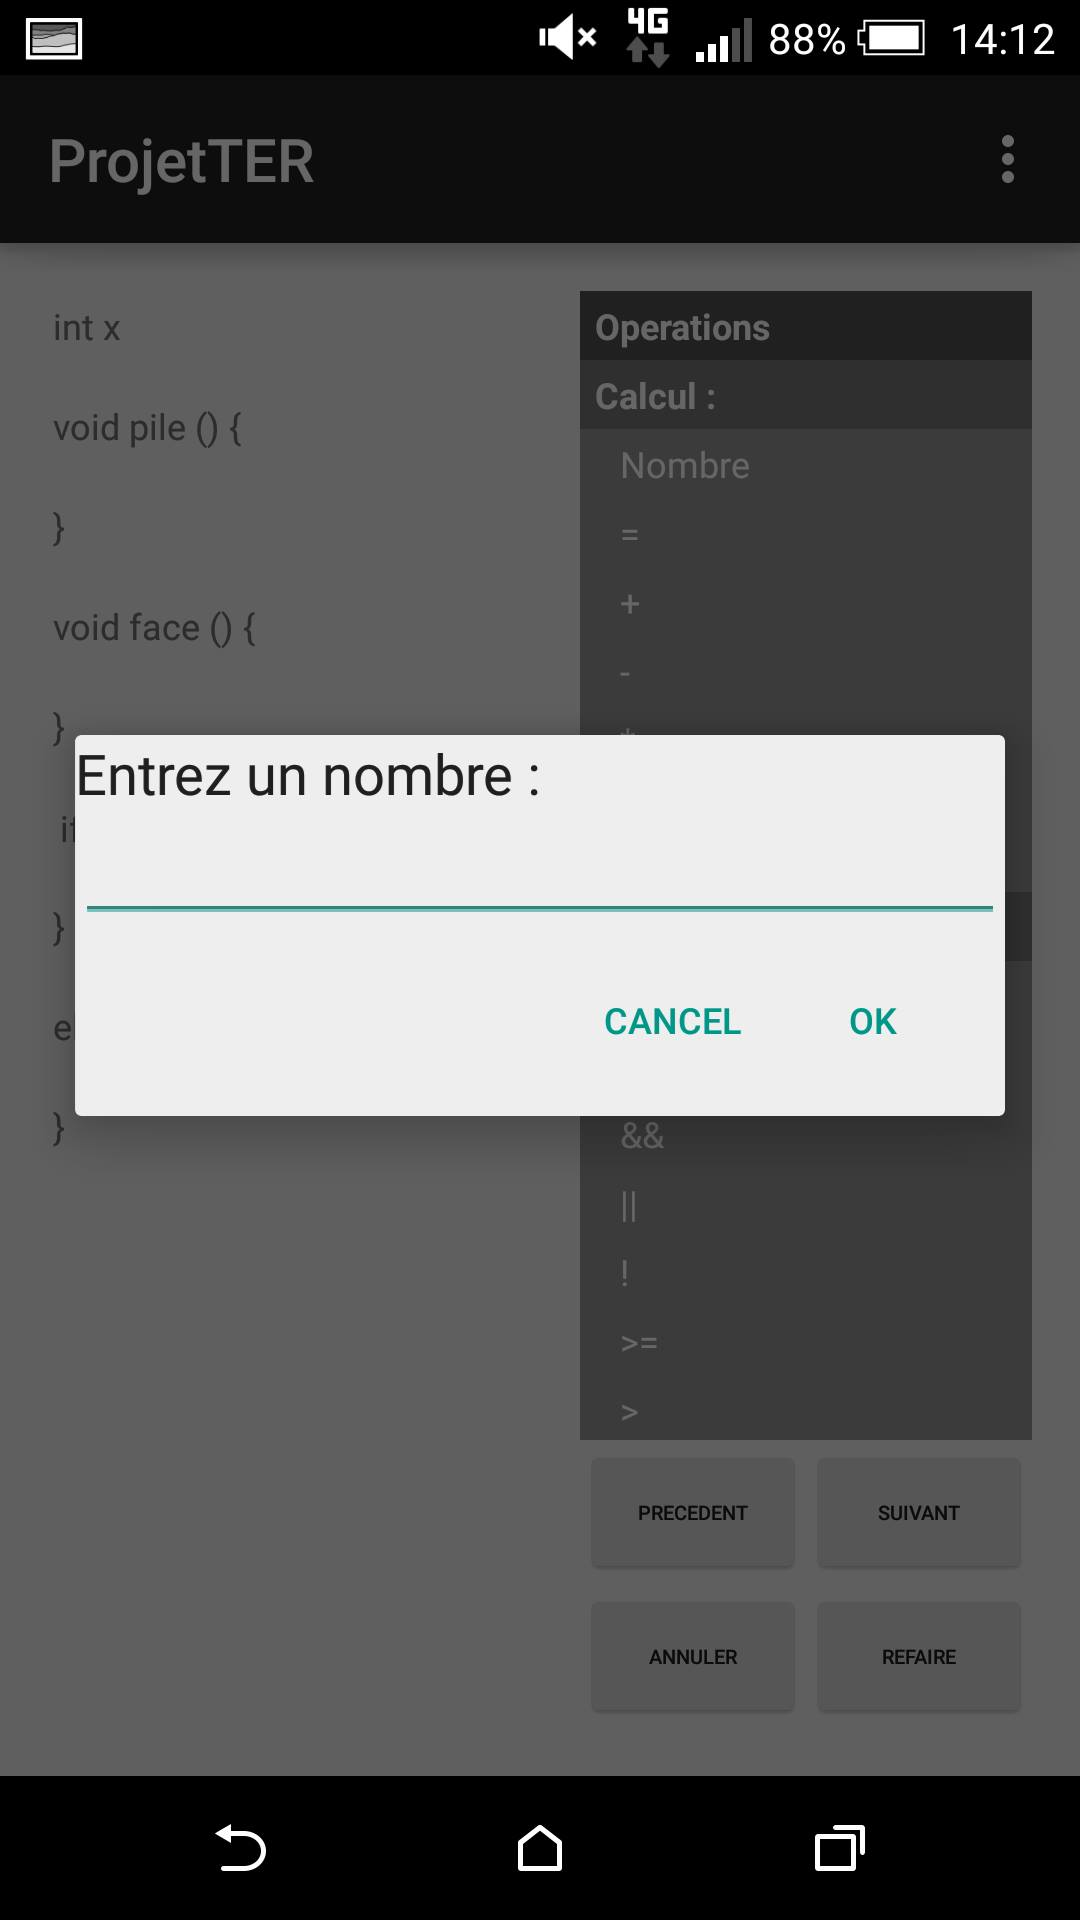
\includegraphics[scale=0.1]{img/popup_nombre.jpg}
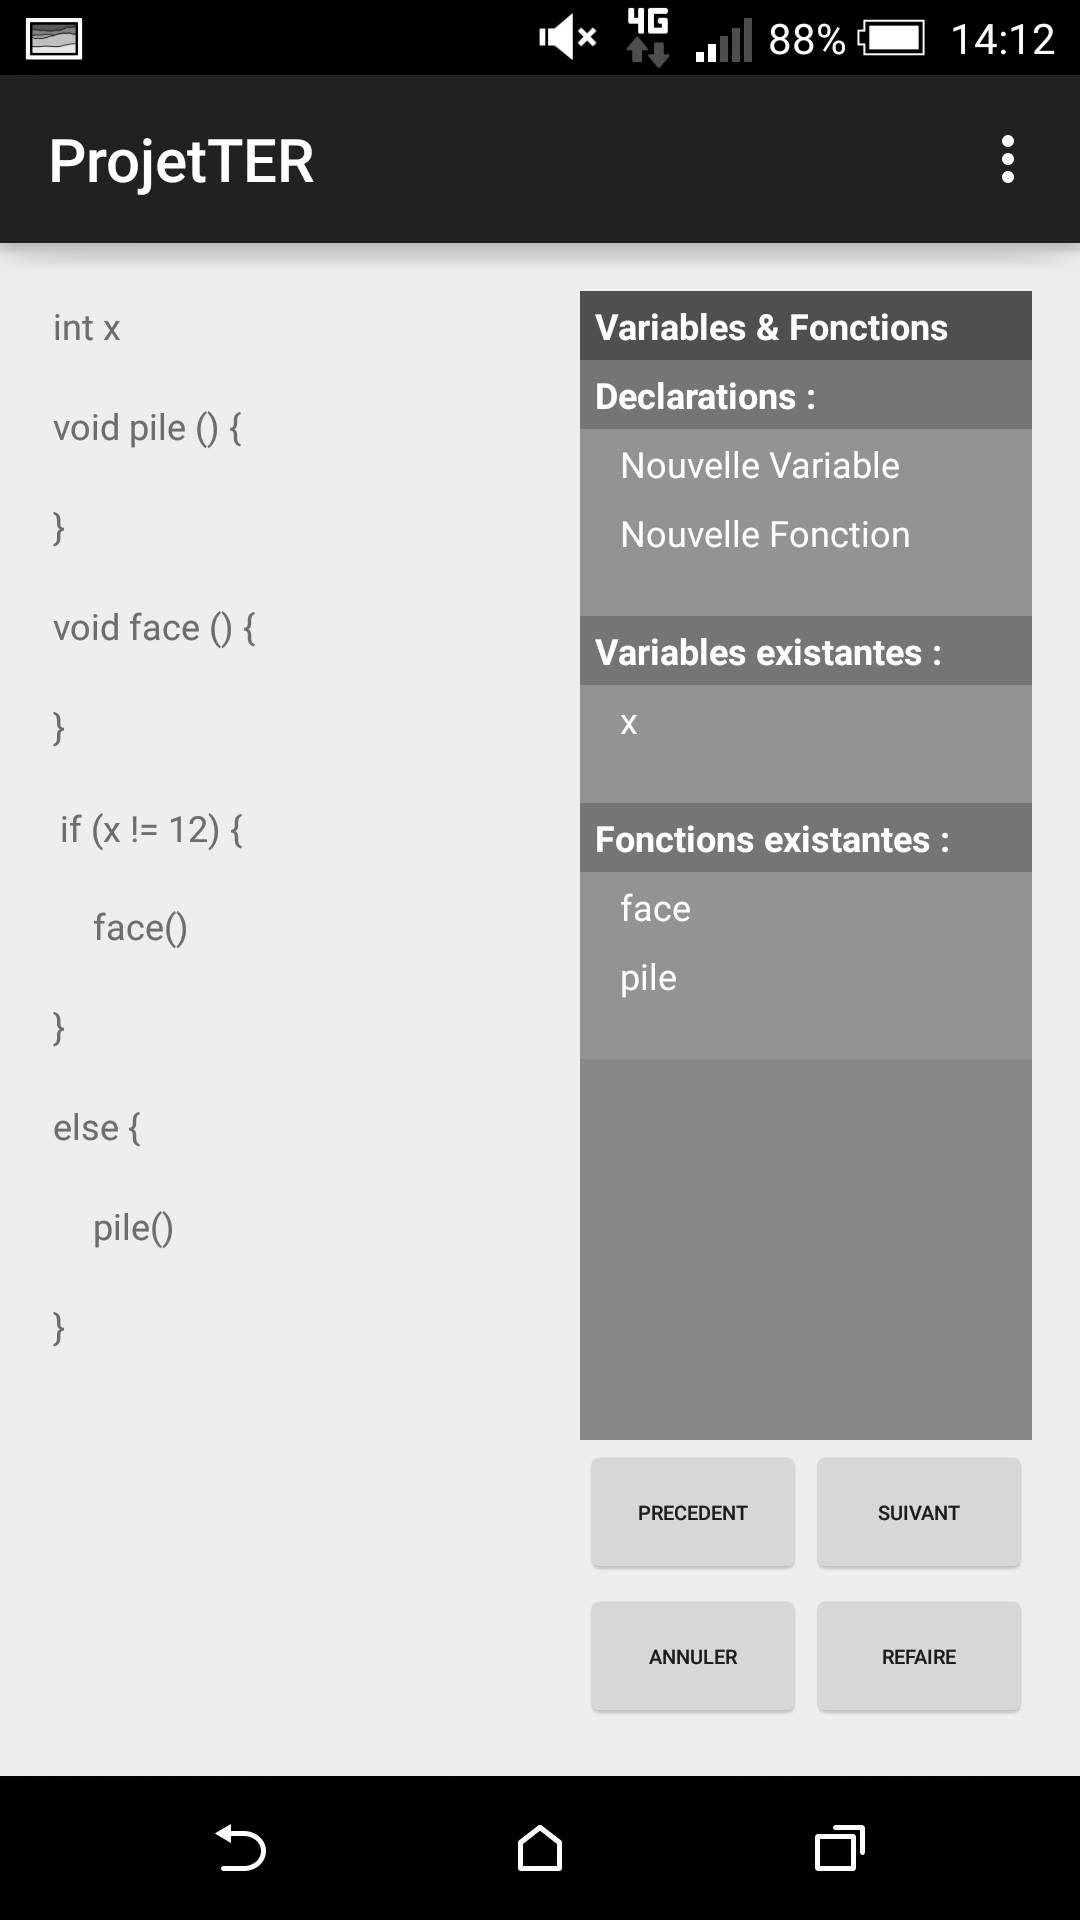
\includegraphics[scale=0.1]{img/create3.jpg}
\end{center}

Scrollview a gauche servant de réceptacle aux éléments de codes. Lors du drag and drop, soit les élément donnent lieu a une nouvelle ligne de code, soit les élément enrichissent les lignes deja présentes (exemple : drop d’une variable dans un if)

\subsection{Prototype robot}

Un code arduino à été écris afin de comprendre des instructions basiques envoyées sur son port serie, et exécute des insctructions en fonctions de la commande reçue.\\
Par exemple, on peut envoyer la suite de commande "w w w a s d" sur le port serie, qui aura pour effet de faire avancer 3 fois pendant 1 secondes le robot vers l'avant, puis de le faire tourner à gauche pendant une seconde, le faire reculer puis tourner à droite pendant une seconde.\\

\paragraph{}
Pour éviter tout dommage sur le robot, des routines dites "de sécurité" sont mises en place dans le code de l'arduino, ces routines permettent d'éviter au robot d'entrer en collision avec tout obstacle présent sur sa route. En effet, le robot verifie en permanence l'espace devant lui, et va chercher à tout prix à éviter la collision avec un obstacle, et cela même si l'instruction du programme qu'il est en train d'éxécuter lui indique d'aller vers cette collision.\\
Cette vérification pourra être désactivée mais sera déconseillée, car un choc à pleine vitesse peut avoir de graves conséquences sur l'intégrité du robot.

\subsection{Prototype compilateur}
Définition d’une grammaire via un outil d’analyse lexicale et sémantique, ATNLR4, qui permet via la description d’expressions régulières combinée de formuler un langage.\\
\\
Une fois cette grammaire définie, l’outil permet de créer un AST, qui permet ensuite d’effectuer l’analyse sémantique via une table des symboles, ce qui aboutira à la production du code machine exécutable sur le robot
\section{Un planning, affectations des tâches}

Victor : mini-langage et compilateur\\
Julien et Vladimir: travail sur l’application\\

\section{exemples de fonctionnement}

\subsection{Matériel}

\paragraph{}
Ce projet implique l’utilisation d’un grand nombre de technologies, en effet, il s‘agit :
\begin{itemize}
\item De designer une interface pour tablette android, compatible avec le maximum de périphériques et de versions d’android, la compatibilité avec une grande palette de taille d’écran est un plus.
\item De charger un programme dans un robot autonome via le réseau, wifi ou bluetooth. il est nécessaire de pouvoir recharger à la volée ces programmes avec un minimum de latences, de ce fait, on laisse place à l’expérimentation.
\item De disposer d’un robot programmable facilement, avec un maximum de moteurs et de capteurs. De ce fait, il sera possible de programmer le robot de manière dynamique avec son environnement, tel une intelligence artificielle, et non une simple suite d’instruction séquentielle.
\item De disposer d’un micro-ordinateur servant à coordonner les différents échanges entre le périphérique de contrôle, la tablette en l'occurrence, et le robot. Ce micro-ordinateur sera de préférence placé directement sur le robot, car relié aux moteurs et capteurs de ce dernier.
\end{itemize}

\paragraph{}
Afin de répondre à toutes ces contraintes, voici le matériel utilisé principalement :
\begin{itemize}
\item La tablette Android de référence pour le développement de l’interface fût une Nexus 7 de 2012 sous Android 5.1.1 Lollipop. Cette tablette possède un écran de 7 pouces, qui est une taille confortable pour la représentation visuelle, tout en étant adaptée à des enfants, un milieu ou une tablette de 10 pouces est plus difficile à manipuler.
\item Notre choix s’est porté sur l’utilisation du réseau wifi, plus stable et plus simple à manipuler que le bluetooth. 
\item La partie programmable du robot est représentée par une carte de type Arduino Leonardo, permettant de contrôler différents périphériques sur des ports de type GPIO tel que des moteurs ou des capteurs infrarouges, la liste des périphériques utilisés est la suivante :
\begin{itemize}
\item 4 moteurs pour chacune des roues, reliées deux par deux, côté gauche et côté droit, ils sont réglables en vitesse via une valeur entre -255 et 255.
\item 1 servomoteur, basé à la tête du robot, permet d’orienter un capteur à ultrasons sur un axe de 0 à 180 de gauche à droite.
\item 1 LED, positionnée directement sur la carte arduino, elle peut être utilisée à vocation de témoin d’une action en cours.
\item 3 capteurs infrarouges, ils sont positionnés à l’avant du robot, un au centre, un à gauche et un à droite. Ils détectent une proximité avec un obstacle (booléen).
\item 1 capteur à ultrasons, basé sur le servomoteur, il permet de mesurer précisément la distance du robot avec un obstacle.
\item 2 odomètres, situés sur chacune des roues arrières, ils mesurent la distance parcourue par chaque roue.
\end{itemize}
\item Le micro-ordinateur est une carte de type pcduino, disposant d’une carte wifi embarquée compatible avec un mode point d'accès qui sera utile lors de l’appareillement avec la tablette. L’OS utilisé est ubuntu, qui permet une large étendue de fonctionnalité.
\end{itemize}

\subsection{Préparatifs}

\paragraph{}
Afin de pouvoir utiliser le programme dans des conditions réelles, il est nécessaire de connecter en wifi la tablette au point d’accès hébergé par la carte pcduino. Le nom de ce point d’accès est “Robotaf”, et pour un souci de simplicité, il ne possède aucun mot de passe afin de pouvoir s’y connecter en 1 geste. 
Une fois connecté à Robotaf, le pcduino est l'hébergeur, son IP est donc déjà connue et il n’est pas nécessaire de la saisir. Pour ce qui est du port choisi il est défini à l’avance afin de permette le téléversement des programmes créés sans aucune configuration.

\subsection{Application android}

\subsubsection{Editeur de code}

\begin{center}
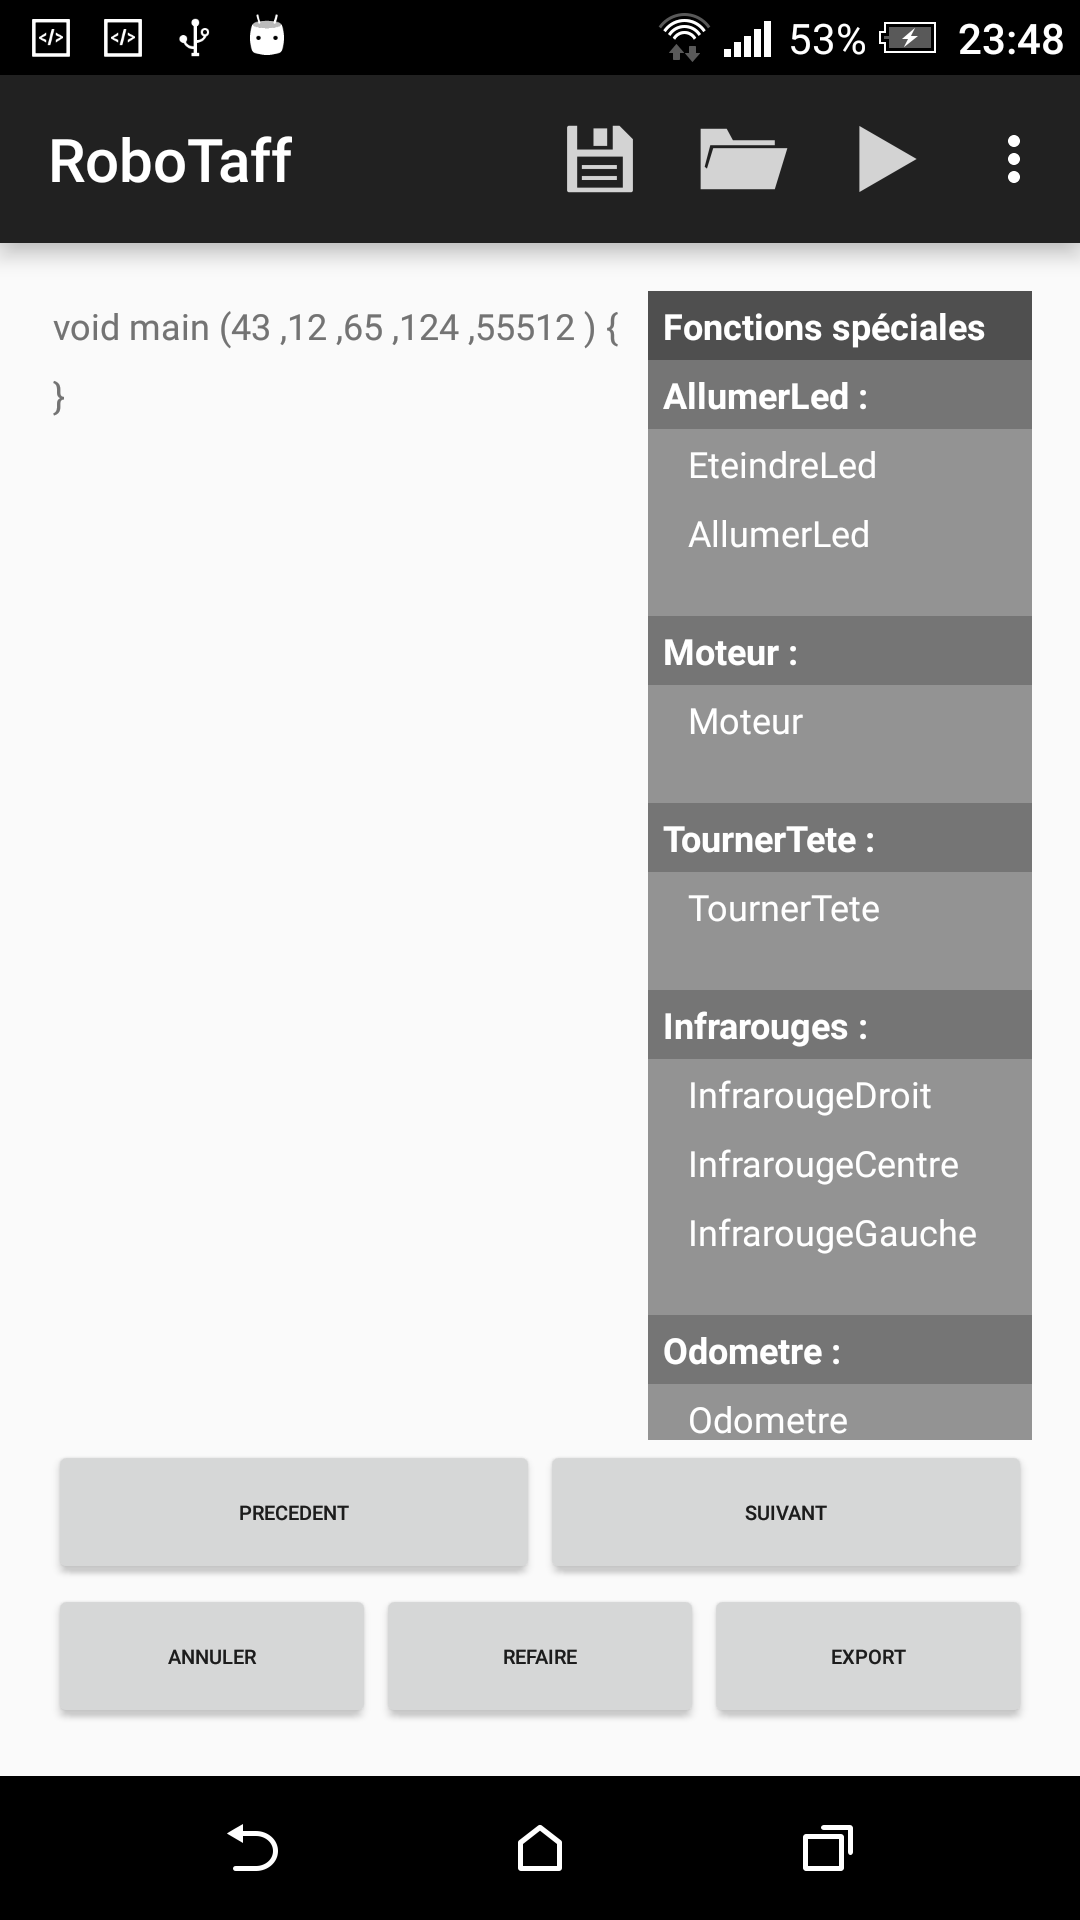
\includegraphics[scale=0.2]{img/main_app.png}
\end{center}

\paragraph{}
Le fonctionnement de l’éditeur de code repose sur le drag'n'drop. On prend des blocks du panel de droite que l’on fait glisser vers la vue centrale, où on pourra crée de nouvelles lignes, ou imbriquer un nouvel élément dans un autre.

\paragraph{}
Lors de l’insertion d’une nouvelle ligne, on colore un en violet un block situé entre deux lignes, par exemple lors de l’insertion d’une nouvelle instruction if, on aura :
\begin{center}
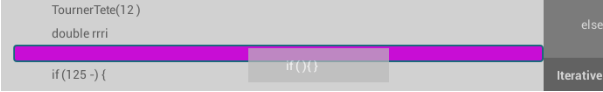
\includegraphics[scale=0.5]{img/edit_1.png}
\end{center}
Génération de 2 nouvelles lignes de code =>
\begin{center}
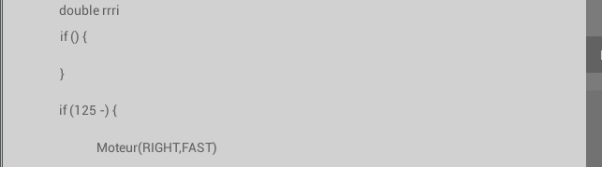
\includegraphics[scale=0.5]{img/edit_2.png}
\end{center}
Lors d’un drag'n'drop sur un block existant, on colore le block pour signaler qu’il est réactif à l’élément qu’on lui présente
\begin{center}
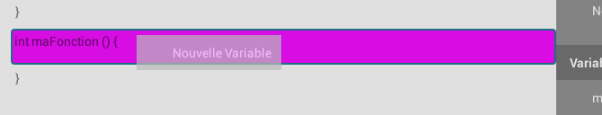
\includegraphics[scale=0.5]{img/edit_3.png}
\end{center}

\subsubsection{Les gestes}
\begin{center}
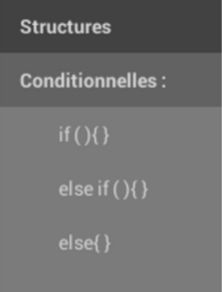
\includegraphics[scale=0.5]{img/gesture.png}
\end{center}

\paragraph{}
Afin d’initialiser le drag'n'drop d’un élément dans le code source, il faut toucher un “MyElement” représenté par les textview en gris clair, puis glisser vers la gauche dans la vue centrale.

\paragraph{}
On laissera déplacer les éléments algorithmiques (Production) de la vue centrale avec le même procédé.\\
De plus, les Productions sont modifiables et supprimable via un LongClick. 

\subsubsection{Sauvegarde Et restauration de contenu}
\begin{center}
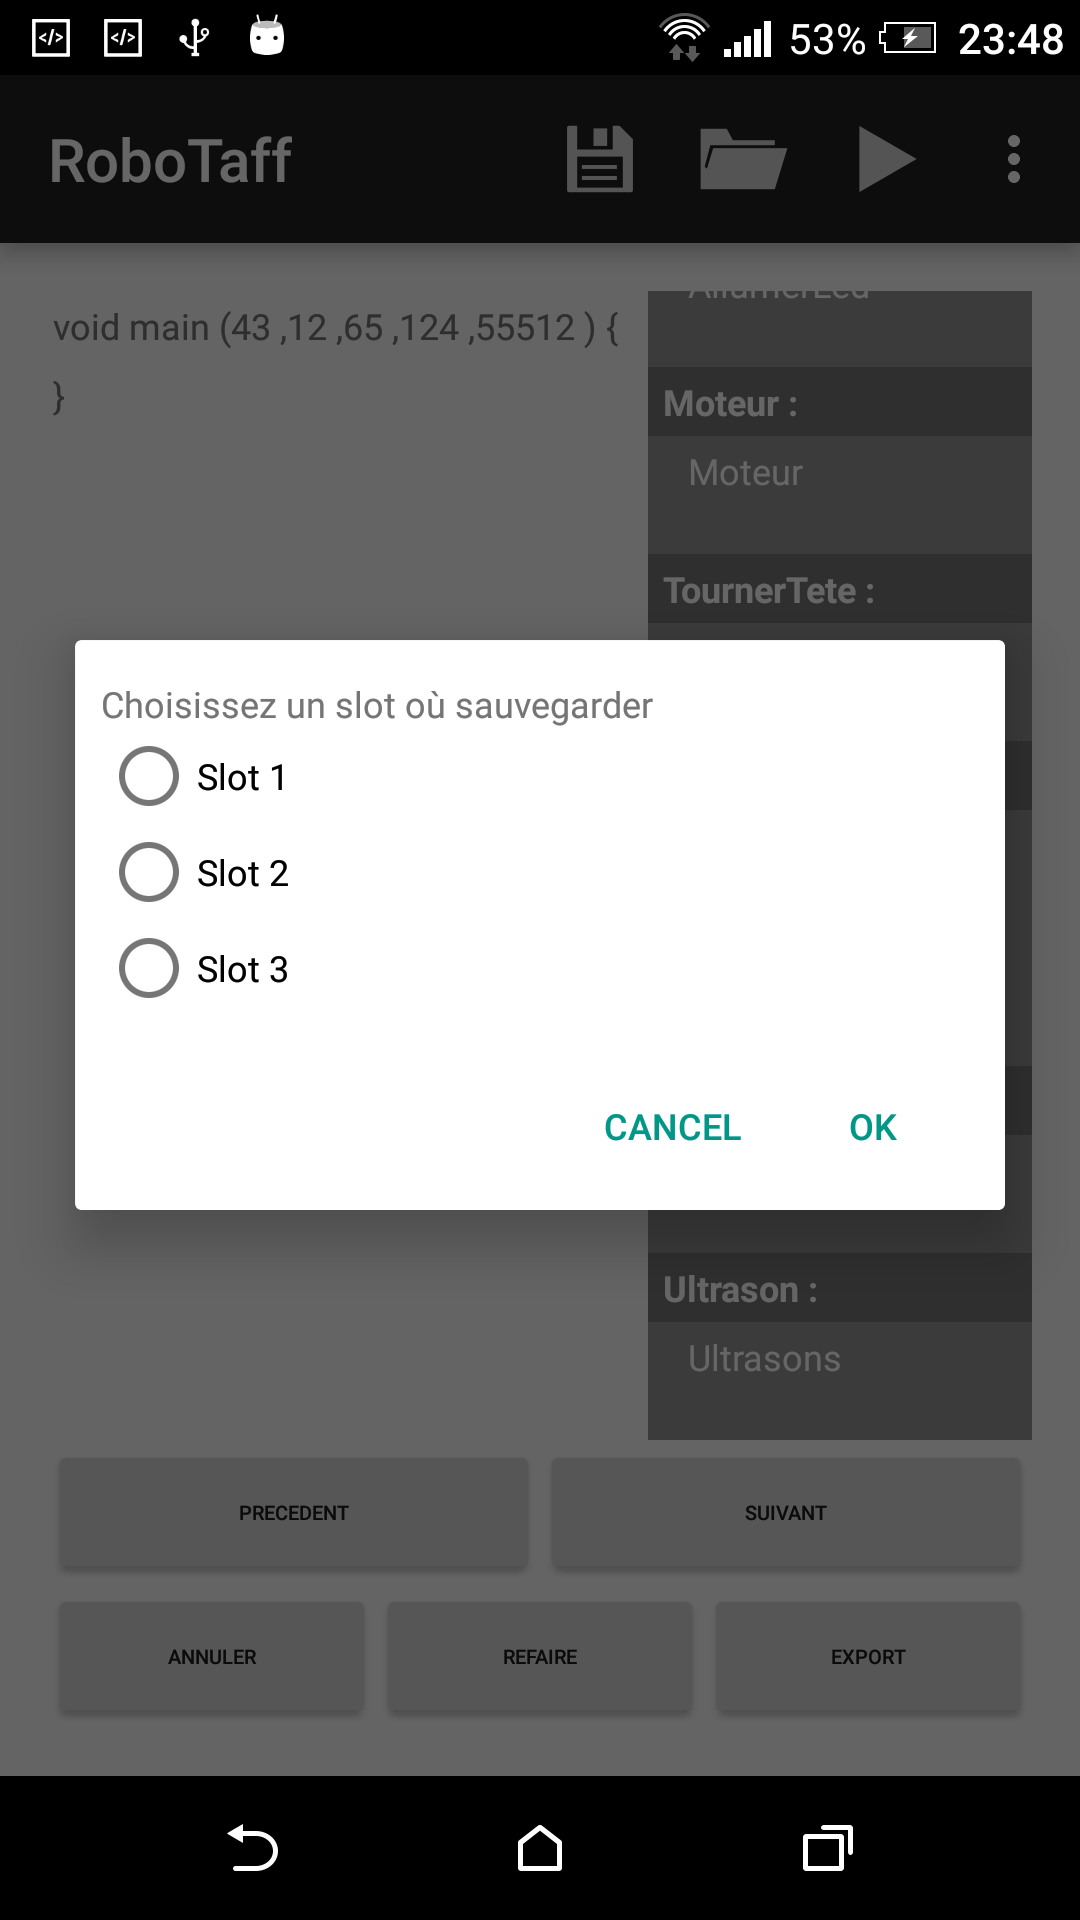
\includegraphics[scale=0.2]{img/save.png}
\end{center}

\paragraph{}
Afin de conserver les algorithmes pour les reprendre plus tard sans devoir les réécrire au lancement de l’application, nous avons mis au point un système de sauvegarde.\\
Ainsi en haut de l’écran dans la barre des actions, nous avons placé deux boutons,
une disquette pour la sauvegarde et un dossier pour le chargement.\\
Aux clics des ces boutons, une popup demande à l’utilisateur de choisir entre les trois slots disponibles pour sauvegarder ou charger son algorithme.

\begin{center}
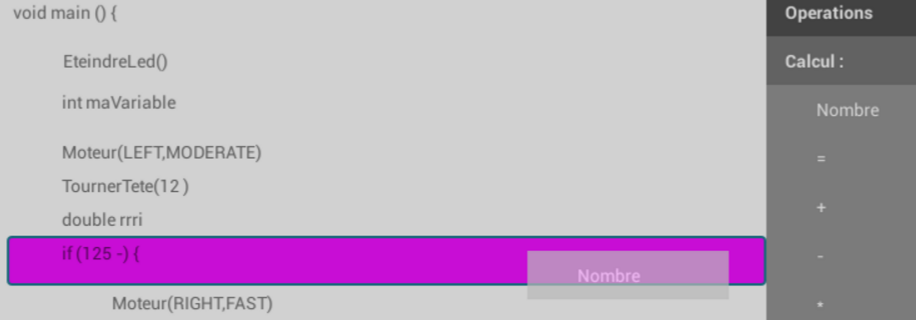
\includegraphics[scale=0.4]{img/edit_4.png}
\end{center}

\paragraph{}
Ici nous avons fait appel à une méthode de sérialisations des données. Le système de sauvegarde enregistre la liste de tous les ElementString de la vue de l'algorithme (objet composé de plusieurs String découlant des objets Production). Ces strings sont sérialisées dans un fichier sur la carte SD de l’appareil, dont le nom dépend du slot.\\
Afin de reconstruire les liens vueAlgorithme-modèle après un chargement, les objets Production sont réinstanciés depuis les ElementString récupérée dans le fichier, via un constructeur.

\section{Architecture}

\subsection{Application  Android}

\subsubsection{Modèle et Vues}

\paragraph{}
Le modèle se base sur l’objet : “ElementString”, qui contient une liste de composant de même type. Les ElementString seront contenu dans des vues, aussi appelées “Production” (de code) qui sont crées à partir d’éléments (“MyElements”) que l’ont met à disposition à l’utilisateur sur le coté droit de l’application.

\paragraph{}
Les éléments (“MyElements”) servant à générer le code, implémentent l’interface “DraggableElement”, où ils donnent des directives afin de pouvoir générer le code final : 
soit en drag'n'droppant sur des lignes vides afin d’en créer de nouvelles, soit en drag'n'droppant sur une ligne déjà existante afin d’ajouter des “ElementString” en argument.

\paragraph{}
Chaque élément de code conventionnel (“if => IfString”,”instanciation de variable=>InstanciationVariableString”, “appel de fonction=>FonctionString”, … ) héritent de ElementString, sachant que chacun définira si il est réactif ou non aux autres éléments. 

\paragraph{}
Par exemple le IfString sera réactif au nombre, variables, etc. En revanche il ne sera pas réactif aux instanciations de variables. Sur l’interface on montre ça en faisant passer la view contenant le IfString (que l’on appellera “Production”) en violet à l’approche d’un élément dont il est réactif.

\subsubsection{Undo - Redo}

\begin{center}
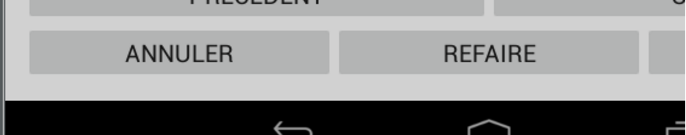
\includegraphics[scale=0.5]{img/undo.png}
\end{center}

\paragraph{}
Concernant toutes les opérations servant à modifier le code source généré, on créé un objet héritant de la classe abstraite “Action” contenant une méthode doAction(), undoAction() où, pour chaque action, on donne des directives sur comment effectuer, et annuler l’action

\paragraph{}
Par exemple concernant l’ajout d’une ligne, on implémente doAction où l’on ajoutera une Production à la vue dédiée au code source, et dans undoAction, on précisera qu’il faut retirer cette même Production de sa vue parente.

\paragraph{}
Les actions sont stockées dans 2 Stack<Action>, appelées undoStack et redoStack.
Ainsi, lors de l’appuie sur l’un des boutons, on pop() l’action d’une Stack, puis on applique sa méthode doAction / undoAction selon le bouton pressé, et on place l’action dans l’autre Stack.

\subsection{Interface et connexion réseau}

\paragraph{}
Nous avons mis en place un serveur Java muni d’un protocole très simpliste, attendant simplement la connexion, puis attendant de recevoir un code source et répondant à l’application le résultat de la compilation de ce code source, qu’elle soit réussie, ou ratée, auquel cas, on enverra les numéros de lignes problématique au compilateur à l’utilisateur. 

\subsection{Compilateur}
\paragraph{}
Une fois le code téléversé sur la carte pcduino, il est sous une forme proche d’un langage impératif classique, or ce type de langage, avec les variables et les structures de contrôles associées tel que les conditions ou les boucles, n’est pas exécutable tel quel sur un processeur. Il est donc nécessaire de traiter le langage reçu pour le convertir en suite linéaire d’instruction, avec des déplacements sous forme de sauts, classiques ou conditionnels. C’est donc la première étape de notre traitement de l’algorithme, la compilation.

\subsubsection{Construction de l’AST}
\paragraph{}
La première étape de la compilation consiste à la création d’un AST, un arbre de syntaxe abstraite qui va permet de représenter le programme sous forme d’arbre. On effectue ainsi une première vérification sur l’intégrité du programme. Cet AST servira de base pour la suite de tout les traitements.

\subsubsection{Construction de la table des symboles}
\paragraph{}
La table des symboles permet de relier toutes les variables et fonctions à un type à un moment donné du programme, cette table sert également à étiqueter chaque variables et fonctions afin de pouvoir y faire référence via son index, notamment lors de l’accès aux registres ou aux frames dans les futurs étapes de la compilation. 

\subsubsection{Conversion vers un langage intermédiaire}
\paragraph{}
La prochaine étape est de linéariser chaque bloc de contrôle afin de n’utiliser qu’un jeu restreint d’instructions classiques, proche de l’assembleur. Dans notre cas, nous n'avons pas à aller jusqu'à l’assembleur car le langage intermédiaire - cette liste d’instructions - sera directement analysé par notre interpréteur qui exécutera notre programme. La liste des instructions utilisées est la suivante :
\begin{itemize}
\item Goto : Permet de sauter à un label défini
\item Label : Étiquette dans le programme, lors de l'exécution chaque label correspond à son index dans la liste d’instruction du programme, de cette façon il est possible de modifier le flux d'exécution du programme en sautant vers un label
\item Jump : Similaire au Goto, mais teste une expression booléenne, l’adresse de saut dépendra du résultat de ce test.
\item Assign : Associe le résultat d’une expression arithmétique à un registre, ici symbolisé par une liste de variable, avec un index qui simule les numéros de registre d’un processeur réel.
\item Call : Appel d’une fonction ou procédure, ces instructions seront notamment utilisées lors de l’appel à des fonctions de contrôle du robot, tel que les capteurs ou les moteurs. Les retours des fonctions peuvent être utilisés lors de tests booléens ou affectés à des variables.
\end{itemize}

\subsection{Interpréteur}
\paragraph{}
L'interpréteur est la partie du processus qui va gérer l'exécution du programme, à la manière d’un processeur avec du code assembleur, il va en effet interpréter chaque instruction de la liste générée précédemment et va agir en conséquence, soit en modifiant le flux d'exécution, en modifiant les variables locales, ou encore en lançant des commandes dans l’interface Erlang afin de directement contrôler le robot.

\subsection{Erlang}
\paragraph{}
L’utilisation d’Erlang est une commodité appréciable fournie par les utilisateurs précèdent du robot. En effet, une interface à déjà été développée afin de contrôler l’intégralité des moteurs et capteurs du robot via la carte arduino. Cette interface, utilisable en java via la librairie prévue par Erlang, permet de contrôler directement l’arduino depuis l'interpréteur, et donc d’utiliser le robot pour l'exécution du programme.

\subsection{Arduino}
\paragraph{}
La carte arduino héberge un code en lien avec l’interface Erlang associée, en effet, la carte attend continuellement des ordres sur le port série, que ce soit l’actionnement d’un moteur ou encore la récupération de la valeur d’un capteur.

\section{Justification structures de données utilisés}
\subsection{Choix esthétiques}
\paragraph{}
La priorité était de faire une interface intuitive, ainsi nous avons imaginé cette interface, compatible portait comme paysage, donnant le plus d’espace possible à l’éditeur d’algorithme.\\
Concernant le style visuel, pour un premier prototype le style devait rester simple et plutôt sobre, néanmoins pour garantir un rendu similaire entre toutes les versions d’Android les méthodes et styles des pages héritent de classes AppCompat/AppCompatActivity, elles garantissent un rendu de type Material Design dès Android 2.3.

\subsection{Choix technologiques}
\paragraph{}
L’idée initiale était de programmer manuellement l’arduino afin de se prémunir du processus erlang en tâche de fond sur le pcduino. Mais il s’est avéré que le gain de temps apporté par l’utilisation de l’interface Erlang n’étais pas négligeable, et cela à permis de se concentrer sur d’autres points du projet, afin de fournir un prototype fonctionnel dans le temps imparti.

\paragraph{}
Pour ce qui est de l’utilisation du compilateur, nous avons profité de celui crée lors du projet de cours de compilation afin de mieux répondre aux attentes du projet, ce compilateur permettait notamment de gérer toutes les fonctionnalités attendu du langage utilisé dans Robotaf. De plus, le fait de s'arrêter au langage intermédiaire permet de simplifier grandement l'implémentation de ce dernier, car la structure de donnée générée est directement utilisable dans l'interpréteur pour l'exécution du programme.

\section{Extensions possibles du logiciel}
\subsection{Nouvelle interface graphique}

\begin{center}
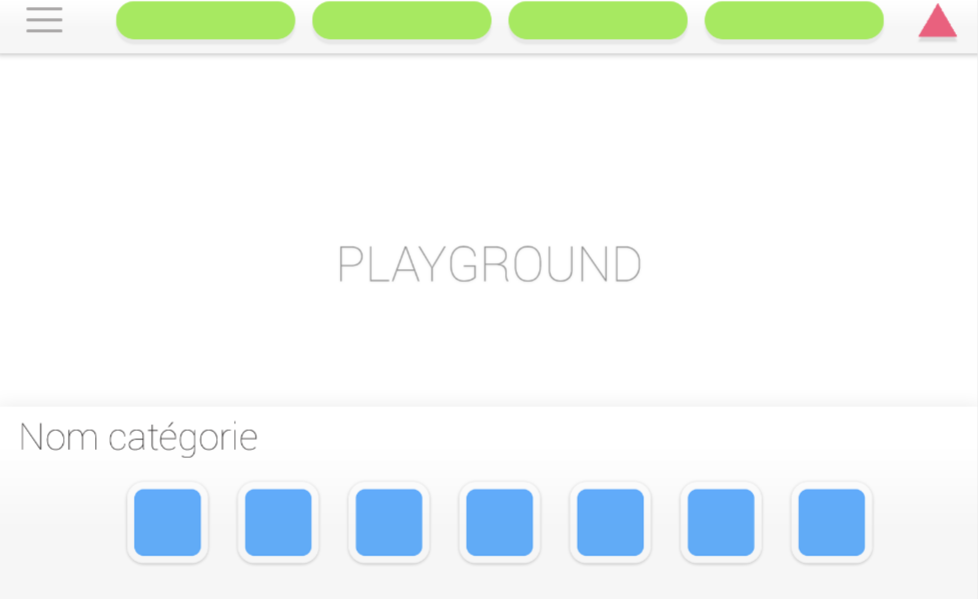
\includegraphics[scale=0.3]{img/new_ui.png}
\end{center}

\paragraph{}
Si dessus une idée d’évolution de l’interface. Au milieu, dans le Playground un Layout sous forme de tableau en 2 dimensions, pouvant recevoir des blocs correspondants à des éléments algorithmiques ou des actions que le robot peut exécuter, ces blocs se trouvent en bas sur le screenshot et seraient classés en catégorie (en haut), on pourrait également penser à un jeu de couleurs facilitant la compréhension des enfants.

\paragraph{}
Ce système serait moins permissif, et permettrait d’éviter l’utilisateur de créer des algorithmes insensés, ou de générer de multiples erreurs.

\subsection{Compilation directe vers l’assembleur}
\paragraph{}
Une possibilité pour une future évolution du projet est la compilation du code vers de l’assembleur natif utilisé par le processeur de l’arduino. En effet, le compilateur utilisé permet de produire du code assembleur, alors pourquoi ne pas directement utiliser ce code produit sur un processeur plutôt que de l'interpréter et de l'interface avec Erlang pour contrôler le robot ? 

\paragraph{}
Nous pensons cette évolution possible, bien que pouvant limiter les approches, car cela rendrais obsolète la carte pcduino, et le code serais directement téléversé sur l’arduino via un shield wifi. D’un autre point de vue, cela ferrait drastiquement chuter le coût de production du robot, car l’on se sépare de sa pièce la plus onéreuse.
Toutefois, cette solution nécessite une maîtrise complète de l’assembleur utilisé sur ce type de carte, avec les fonctionnalités d’accès aux pins GPIO pour contrôler les différents périphériques reliés.

\subsection{Nouveaux capteurs, nouveaux robot}
\paragraph{}
L’architecture évoquée précédemment permet d’investir l’argent économisé avec la carte pcduino dans de nouveaux capteurs ou actuateurs du robot, afin d’augmenter ses possibilités ludiques. On peut ainsi imaginer des lumières, buzzers ou autre caméra toujours contrôlable depuis l’interface de l’application sur la tablette. \\
Par exemple ajouter une boussole au robot permettraient de mieux gérer l’espace, sachant que actuellement, il est impossible de tourner le robot de manière précise du fait de l’adhérence variante du sol.\\
La suppression de la carte pcduino, outre le gain dans le prix du robot, offre un gain de place non négligeable, ce qui permet par la suite d’opter pour un châssis plus compact afin de produire des robots plus adaptés à des espaces confinés.

\vfill\eject
\bibliographystyle{plain}
\bibliography{rapport}
\end{document}
